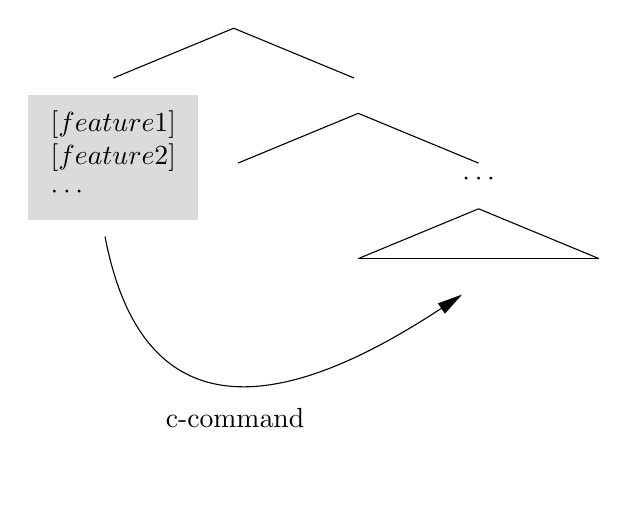
\begin{tikzpicture}[x=0.75pt,y=0.75pt,yscale=-1,xscale=1]
    %uncomment if require: \path (0,300); %set diagram left start at 0, and has height of 300
    
    %Shape: Rectangle [id:dp9128325136098152] 
    \draw  [draw opacity=0][fill={rgb, 255:red, 74; green, 74; blue, 74 }  ,fill opacity=0.2 ] (17,92) -- (99,92) -- (99,152.33) -- (17,152.33) -- cycle ;
    %Straight Lines [id:da30758700085469415] 
    \draw    (58,84) -- (116,60) ;
    %Straight Lines [id:da846606209202029] 
    \draw    (174,84) -- (116,60) ;
    %Straight Lines [id:da11288178549535077] 
    \draw    (118,125) -- (176,101) ;
    %Straight Lines [id:da6959666805958957] 
    \draw    (234,125) -- (176,101) ;
    %Straight Lines [id:da8450684064767249] 
    \draw    (176,171) -- (234,147) ;
    %Straight Lines [id:da17050469547416802] 
    \draw    (292,171) -- (234,147) ;
    %Straight Lines [id:da9273911312638281] 
    \draw    (176,171) -- (292,171) ;
    %Curve Lines [id:da8541881958411093] 
    \draw    (54,160.33) .. controls (77.76,285.07) and (183.85,216.73) .. (224.78,189.16) ;
    \draw [shift={(226,188.33)}, rotate = 145.98] [fill={rgb, 255:red, 0; green, 0; blue, 0 }  ][line width=0.08]  [draw opacity=0] (12,-3) -- (0,0) -- (12,3) -- cycle    ;
    
    % Text Node
    \draw (58,97.4) node [anchor=north] [inner sep=0.75pt]    {$ \begin{array}{l}
    \left[\text{feature 1}\right]\\
    \left[\text{feature 2}\right] \\
    \cdots
    \end{array}$};
    % Text Node
    \draw (234,128.4) node [anchor=north] [inner sep=0.75pt]    {$\cdots $};
    % Text Node
    \draw (82,242) node [anchor=north west][inner sep=0.75pt]   [align=left] {c-command};
    \end{tikzpicture}    